\documentclass[a4paper,12pt,titlepage, twoside, openright, cleardoubleempty]{scrreprt} %page-size, letter-size, with title, is an article

\usepackage[ngerman, english]{babel} %all inserted strings will be german
\usepackage{a4wide} %for better viewing of a4 pages
\usepackage{amsmath}
\usepackage{amssymb}

\usepackage{ntheorem}

\usepackage[T1]{fontenc} %T1-encoded fonts: auch Wörter mit Umlauten trennen
\usepackage{lmodern}
\usepackage[latin1]{inputenc} %letter-style like input � or � possible

\usepackage{vmargin} %Seitenränder einstellen leichtgemacht
\usepackage{fancyhdr} %definiere einfache Headings (mindestens V 1.99c notwendig)

\usepackage{float} %to be able to insert graphics with [H] Options
\usepackage{makeidx} %so the \printindex works

\usepackage{pst-all} %pretty good drawing kit

\usepackage{listings}

\usepackage[vlined,boxed]{algorithm2e}

\usepackage[normalem]{ulem}

\lstset{basicstyle=\ttfamily,breaklines=true}

\usepackage{remreset} %folgende Zeilen benötigt, damit Fußnoten sich nicht zurücksetzen bei neuem Kapitel
\makeatletter
\@removefromreset{footnote}{chapter}
\makeatother 

\lstset{breaklines=true}
\lstset{basicstyle=\ttfamily}
\lstset{language=Java}
\lstset{tabsize=4}

\setcounter{secnumdepth}{3}% Numerierung auch für \subsubsection
\setcounter{tocdepth}{3}% nimm auch \subsubsections ins Inhaltsverz. auf

\clubpenalty = 10000
\widowpenalty = 10000
\displaywidowpenalty = 10000

\setpapersize{A4}
\setmarginsrb{3cm}{1cm}{3cm}{1cm}{6mm}{7mm}{5mm}{15mm}

%% Stil
\parindent 0cm                     % Absatzanfang wird nicht eingerückt
\parskip1.5ex plus0.5ex minus0.5ex % Abstand zwischen zwei Absätzen

\newtheorem{Def}{Definition}

\pagestyle{fancy}
\renewcommand{\chaptermark}[1]{\markboth{\thechapter.\ #1}{}}
\fancyhf{} % clear all header and footer fields
\fancyhead[LE,RO]{{\headfont\thepage}} % left/right header for even/odd pages
\fancyhead[LO]{\headfont\nouppercase{\rightmark}} % header for left side (odd)
\fancyhead[RE]{\headfont\nouppercase{\leftmark}} % right header for even pages
\renewcommand{\headrulewidth}{0.5pt} % head rule
\renewcommand{\footrulewidth}{0pt} % no rule
% plainstyle
\fancypagestyle{plain}{%
\fancyhf{} % clear all header and footer fields
\renewcommand{\headrulewidth}{0pt}
\renewcommand{\footrulewidth}{0pt}
}

\usepackage[pdftex]{graphicx}
\usepackage[pdftex,
bookmarksnumbered,
bookmarks,
bookmarksopen,
bookmarksopenlevel=1,
hypertexnames,
breaklinks,
]{hyperref}
\hypersetup{
pdftitle    = {Titel},
pdfsubject  = {...},
pdfauthor   = {},
pdfkeywords = {},
colorlinks  = {false},
linkcolor   = {blue},
citecolor   = {cyan}
}
\pdfcompresslevel=9
\pdfinfo{
/CreationDate (D:2015 11 24 00 00 00) % year(4) month(2) day(2) hour(2) minute(2) second(2)
/ModDate      (D:2015 11 24 00 00 00) % modification date
}

%%%%%%%%%%%%%%%%%%%%%%%%%%%%%%%%%%%%%%
%%%%%%%%%%%%%%%%%%%%%%%%%%%%%%%%%%%%%%
%%%%%%%%%%%%%%%%%%%%%%%%%%%%%%%%%%%%%%
%%% Hier die richtige Trennung von Wörtern festlegen, die Latex sonst 
%%% falsch trennt.
%%%%%%%%%%%%%%%%%%%%%%%%%%%%%%%%%%%%%%
%%%%%%%%%%%%%%%%%%%%%%%%%%%%%%%%%%%%%%
%%%%%%%%%%%%%%%%%%%%%%%%%%%%%%%%%%%%%%
\hyphenation{Media-annotation}


\makeindex %must be before "begin{document}
\begin{document}
\graphicspath{{pics/}}

\pagestyle{empty}

\pagenumbering{roman}

%%%%%%%%%%%%%%%%%%%%%%%%%%%%%%%%%%%%%%
%%% Titelseite
%%%%%%%%%%%%%%%%%%%%%%%%%%%%%%%%%%%%%%
\selectlanguage{ngerman}
\begin{titlepage}
\begin{singlespacing}
\begin{center}
\begin{flushleft}
	University of Passau\\
	Faculty of Computer Science and Mathematics
\end{flushleft}

\begin{center}

\vspace{1.0cm}


\includegraphics[width=7cm]{figures/uni-logo.png}

\vspace{2.5cm}


\Large{Bachelor thesis}

\vspace{1.0cm}

\begin{doublespace}
\textsf{{\Huge\textbf{\thetitle}}}
\end{doublespace}

\vspace{1.0cm}

{\bfseries \Large{\theauthor}}

\vfill
\end{center}

%%% oder:
% \date{<schreib_irgendwas_rein>}


\vspace{3.0cm}

\normalsize
\begin{flushleft}
\begin{tabular}{ll}
\multicolumn{2}{l}{Bachelor thesis}\\
\multicolumn{2}{l}{Chair of Distributed Information Systems}\\
\multicolumn{2}{l}{Faculty of Computer Science and Mathematics}\\
\multicolumn{2}{l}{University of Passau}\\
\\
%%%%%%%%%%%%%%%%%%%%%%%%%%%%%%%%
%%% Falls Diplomarbeit - bei BA nur ein Gutachter im Moment
%%%%%%%%%%%%%%%%%%%%%%%%%%%%%%%%
Examiner: & Prof. Dr. Harald Kosch \\
Supervisor: & Armelle N. Ndjafa
\end{tabular}
\end{flushleft}

\parbox{\linewidth}{\hrule\strut}

\thedate

%\dedication{Widmung}
\end{center}
\end{singlespacing}
\end{titlepage}

\pagestyle{fancy}
\selectlanguage{english}

%%%%%%%%%%%%%%%%%%%%%%%%%%%%%%%%%%%%%%
%%% Kurzfassung (wenn möglich auf Englisch, ansonsten Deutsch)
%%%%%%%%%%%%%%%%%%%%%%%%%%%%%%%%%%%%%%
\chapter*{Abstract}

Health care faces the problem of dealing with a vast amount of heterogenous data, that isn't easily accessible. Classical data integration approaches need a global schema before queries on the integrated data can be stated. Dataspace is a new abstraction of data management, that doesn't enforce any schema, allows data-coexistence, and needs only low upfront work for datasources thus being suitable for highly heterogeneous environments. In this thesis we present MeDSpace, a distributed system that allows to state keyword search queries over heterogeneous datasources. The presented system is a test environment for medical datasources and can be used as a starting point for creating a dataspace over multimedia datasources. The system uses medical data, but could be used for any kind of multimedia data that should be searchable by keywords.

%%%%%%%%%%%%%%%%%%%%%%%%%%%%%%%%%%%%%%
%%% Inhaltsverzeichnis
%%%%%%%%%%%%%%%%%%%%%%%%%%%%%%%%%%%%%%
\tableofcontents

\cleardoublepage %beginne neue Seitenzählung auf einer rechten Seite (ungerade Seitenzahl)

%%%%%%%%%%%%%%%%%%%%%%%%%%%%%%%%%%%%%%
%%% Tabellenverzeichnis
%%%%%%%%%%%%%%%%%%%%%%%%%%%%%%%%%%%%%%
\listoftables
\addcontentsline{toc}{chapter}{List of Tables}

%%%%%%%%%%%%%%%%%%%%%%%%%%%%%%%%%%%%%%
%%% Abbildungsverzeichnis
%%%%%%%%%%%%%%%%%%%%%%%%%%%%%%%%%%%%%%
\listoffigures
\addcontentsline{toc}{chapter}{\listfigurename}

%%%%%%%%%%%%%%%%%%%%%%%%%%%%%%%%%%%%%%
%%% Diese beiden Zeilen werden für Doppelseitigen Ausdruck benötigt und
%%% damit erst nach dem Inhaltsverzeichnis die Seiten gezählt werden.
%%%%%%%%%%%%%%%%%%%%%%%%%%%%%%%%%%%%%%
\cleardoublepage
\pagenumbering{arabic}

%%%%%%%%%%%%%%%%%%%%%%%%%%%%%%%%%%%%%%
%%% Ab hier beginnt die eigentliche Arbeit.
%%%
%%% 2 Varianten:
%%%     - entweder einzelne Kapitel mit include einbinden (bessere Übersicht)
%%%     - oder den ganzen Text einfach reinschreiben (unübersichtlich)
%%% Wie es gemacht wird spielt fürr den eigentlichen Output keine Rolle.
%%%%%%%%%%%%%%%%%%%%%%%%%%%%%%%%%%%%%%
%%%% Part dient dazu, zb. die Arbeit nochmal zu Gliedern (Einleitung, Theorieteil, ...)
\part{Part}

% neues Kapitel
\chapter{Chapter}

Always make a short intro to chapters or sections.

%neue Section
\section{Section}
\label{erstesLabel}

some intro words \dots

% NICHT TIEFER ALS SUBSECTION!!!
\subsection{SubSection}
\label{zweitesLabel}

First label was set in section \ref{erstesLabel} - the second in section \ref{zweitesLabel}.

Remember: Always reference any figures or tables within the prose text!

A reference will be done like this: \cite{keyToBibEntry}

Do not cite things like Wikipedia, Slides, etc (only Books and scientific papers allowed - or W3C Recommendations \cite{w3c_example} and articles on trusted sites marked with a date and an corresponding author)

Please code URLs like this: \url{http://www.google.de}

If you name projects like A.I.R\footnote{\url{https://www.dimis.fim.uni-passau.de/iris/index.php?view=air} -- last checked: \today} or Eclipse\footnote{\url{http://www.eclipse.org/} -- last checked: \today} or whatever, use footnotes to cite the URL.

%Example Figure
\begin{figure}[H]
	\begin{center}
		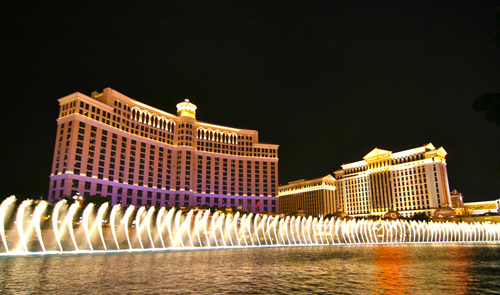
\includegraphics[width=0.75\textwidth]{holiday.png}
	\end{center}
	\caption{After the thesis it's time for holiday}
	\label{labelToRef}
\end{figure}

%Example Itemize
\begin{itemize}
	\item item 1
	\item item 2
	\item lala
\end{itemize}

%Example Description
\begin{description}
	\item[item 1] is needed in order to blabla
	\item[item 2] defines blabla
	\item[lala] lala
\end{description}

% Example Definition
\begin{Def}[Title]
\label{key}
Description \dots
\end{Def}

% Example Table
\begin{table}[H]
\begin{center}
\caption{Caption of the table}
\label{lalala}
\begin{tabular}{| l | l |}
\hline
first column & second column \\
\hline
\hline
\dots & \dots \\
\hline
\dots & \dots \\
\hline
\end{tabular}
\end{center}
\end{table}

\begin{procedure}[ht]        
\caption{Greedy Heuristic()} 
\label{greedy}        
\KwData{request profile $Q$, backends $B$} 
\KwResult{allocation schema}

sort(request profile $Q$) according cost function $c_S$ descending \; 

\ForEach{$C \in Q$}{

   \ForEach{$b \in B$}{
      \eIf{$b.free\_capacity > 0$} {
      $UNION \leftarrow b.relations \cup C.relations$\;
      $INTERSECT \leftarrow b.relations \cap C.relations$\;
      ${diff}[C,b] \leftarrow c_S(INTERSECT) - c_S(UNION)$\;
      }
      {$diff[C,b] \leftarrow -\infty$;}
   }
   
   \While{$C.rest\_workload > 0$}{
      
      $b \leftarrow b \in B \mbox{ where } diff[C,b]  \mbox{ maximal}$\;
      
      $workload\_for\_b \leftarrow \min({b.free\_capacity, C.rest\_workload})$\;
      
      $b.add(C , workload\_for\_b)$\;
      
      $C.rest\_workload \leftarrow C.rest\_workload - workload\_for\_b$\;
      
      
      ${diff}[C,b] \leftarrow -\infty$;
      
   }
}
\end{procedure}


%\include{summaries/summaries}
\section{Towards a Model for Multimedia Dataspaces}

In the paper 'Towards a Model for Multimedia Dataspaces'\cite{6167826} the authors present a representation model for dataspaces, which is an approach based on the dataspace and dataspace-view paradigm for uniformly represent  structured and semi structured data, ontologies and other similar knowledge representation models. 
With that model, the authors address the current explosion of digital information and data sources. Many branches (i.a. in the medicine) need now large amounts of distributed, heterogeneous data. 

However, traditional data integration methods are barely applicable to formulate search queries on a distributed,  heterogeneous data set, containing files with many different file formats, as traditional data integration systems are designed for complete structured data.
Thus, these systems need a global schema for calculating search queries. 
Addressing this issue, the concept of dataspaces was developed as an abstraction of wide-area, heterogeneous and distributed data management.
For dataspaces there is no need of upfront efforts to semantically integrate data before basic services such as keyword search can be provided. 

Dataspaces support uncertainties in schema-mapping and consider that schema mapping from sources to  mediated schema may be incorrect.
A further interesting feature of dataspaces is successive data integration. So, the system is able to  integrate data in iterations as the time goes on depending on user needs.

Research in the field of dataspaces is currently very active, but despite of the deep interest, existing models suffer on a number of shortcomings limiting their applicability.
These include the tendency of overlooking the different types of relations that can exist between data items, which restricts the amount of information they can generally integrate.
Second, they focus on classical text data ignoring the specifics of multimedia data. Third they don't provide the fine-granularity in the persistence of integrated data that is needed in certain domains.

To address these issues, the authors developed a dataspace model, which sees the dataspace as a set of classes, objects (instances of classes) and relations.
In the latter case there exist relations between classes (CRC), relations between objects and classes (ORC) and relations between objects (ORO).
Furthermore relations can be internal or external defining whether the anticipating relation objects are in the same data source or in different ones.

A design goal of the model is the maximization of its expression in terms of the types of relations that it can represent, enabling it to deal with information originating from structured data, semi-structured data, ontologies and other forms of knowledge representation as well as from canonical  
knowledge.

Import to note is the fact that the model includes similarity relations in the type of relations. 
Similarity functions are a feature of multimedia data that defines a measurement for non-exact matching between objects.
This kind of relations can be used to derive relations between other objects in the dataspace.
Additionally the model introduces the concept of dataspace-view. 
This makes it possible to store query results of an existing dataspace into a new sub-dataspace with different modes of persistence(virtualized view, materialized view, mode of synchronization with the content of the original sources,...).\\
\section{Databases to Dataspaces - A New Abstraction for Information Management}

Dataspaces describes a new abstraction of data management \cite{Franklin:2005:DDN:1107499.1107502}. In current scenarios it is rarely the case, that data to be managed is solely stored in a convenient relational Database Management System (DBMS) or in another, single data model. Therefore, developers often face the challenge to deal with heterogeneous data on a low level base. Challenges are to provide search and query capabilities, enforcing rules, integrity constraints, naming conventions etc.; tracking lineage; providing availability, recovery and access control; and managing evolution of data and meta-data. That issues are ubiquitous and arise in enterprises, government agencies and even on one's PC desktop. 

As a response to this problem, the authors postulate the concept of dataspaces and corresponding to this, the  development of DataSpace Support Platforms (DSSPs). Shortly said, the latter provides an environment of cooperating Services and guaranties, that enables software developers to concentrate on their specific application problem rather than taking care of returning issues in consistency and efficiency of huge, linked but heterogeneous data sets. The remarkable properties of a dataspace system are defined as follows:

A DSSP must deal with data and applications in a variety of file formats, that are accessible through many systems with different interfaces. A DSSP has to support all kinds of data in the dataspace rather than only a few (as DBMSs do).
Although a DSSP provides a integrated possibility for searching, querying, updating and administration, the data often can only be accessible and modifiable through native interfaces. Therefore DSSPs haven't full control over their data.
Queries on a DSSP may offer varying levels of services. In some cases the answers can be approximated resp. best-effort. An example: If some data sources are unavailable for some reasons the DSSP is able to return the best result as possible. Therefore it uses the data that are available at the time of the query.
A DSSP has to provide the tools that allow a tighter data integration process in the dataspace as necessary.

Many of the services a dataspace provide, data integration and exchange systems provide, too. The main difference between these systems is that data integration systems need a semantic integration process before they can provide any services on the data. But dataspace is not kind of a classic data integration approach. In order to avoid semantic integration, a dataspace uses the concept of data coexistence.  The idea is to provide base functionality over all data sources, regardless of their specific integration constraints. E.g. a DSSP is able to provide a keyword search similar to a desktop file search. If more sophisticated operations are required such as relational queries, data mining or monitoring of specific data sources, additional effort can be done to integrate the sources tighter. This incremental process is also called as ``pay-as-you-go'' fashion.

In chapter 3 of the paper the authors pottered at the logical components and services a DSSP should have:

\textbf{Logical components}

A Dataspace should contain all information being relevant for a specific organization/task regardless of their file format or storage location, and it should model a collection of relationships between the data repositories. Therefore the authors define the dataspace as a set of participants and relationships. Participants of a dataspace are individual data sources . Some participants support expressive query languages for querying while others only provide limited access interfaces. Participants can reach from structured, semi-structured right up to unstructured data sources. Some sources provide traditional updates, some are only be appendable, while others are immutable. Further, dataspaces can be nested within each other, which means that a dataspace should be able to be a part of another dataspace.  Thus, a dataspace has to provide methods and rules for accessing its sub dataspaces.

\textbf{Services of dataspaces}

The most basic services a dataspace should contain is the cataloging of data elements of all participants. A catalog is an inventory of data resources containing all important information about every element (source, name, storage location inside the source, size, creation date, owner, etc.)of the dataspace. It is the infrastructure for the most other dataspace services. Search and query are two main services a DSSP must provide. A user should be able to state a search query and iteratively precise it, when appropriate, to a database-style query. For the dataspace approach it is a key tenet that search should be applicable to all of the contents, regardless of their formats.
The search should include both data and meta-data. The user should be enabled to discover relevant data sources and inquire about the completeness, correctness and freshness. A DSSP in fact should be aware of the gaps in its coverage of the domain.  
A DSSP should also support updating data. Of course, the mutability of the relevant data sources determines the effects of updates.  
Other key services would be monitoring, event detection and the support for complex workflows (e.g. it is desired that a calculation is done if new data arrives and that the result will be distributed over a set of data sources). On a similar way a DSSP should support various forms of data mining and analysis. 
Not every participant will provide all necessary interfaces for being able to support all DSSP features. Hence it is necessary, that data sources can be extended on various ways. E.g. a source don't store its own meta-data, so there has to be an external meta-data repository for it. 

\textbf{Components and architecture of a dataspace system}

\uline{Catalog and Browse} Information about all participants and the relationships among them are stored in the catalog. It must also deal with a large variety of sources and supports to provide different levels of information about their structure and capabilities. It is important, that the catalog includes the schema of the source, statistics, rates of change, accuracy, completeness query answering capabilities, ownership, and access and privacy policies for each participant. Relationships may be stored as query transformations, dependency graphs or even textual descriptions. If possible, the catalog should include a basic inventory of the data elements at each participant: identifier, type, creation data and so forth. Then, it can support basic browsing over the participant's inventories.
It isn't a very scalable interface, but it can be used to response to questions about the presence or absence of a data element, or determine which participants have documents of a specific type. 
On top of the catalog, the DSSP should have a model-management environment allowing the creation of new relationships and manipulation of existing ones.

\uline{Search and Query} The component has to offer the following capabilities:

(1) \emph{Query everything:} Any data item should be queryable  by the user regardless of the file format or data model. Keyword queries should be supported, initially. When more information about a participant is collected, it should be possible to gradually support more sophisticated queries. The transition between keyword query, browsing and structured querying should be gracefully. And when answers are given to keyword (or structured) queries, the user should be able to refine the query through additional query interfaces. 

(2)\emph{Structured query:} Queries similar to database ones should be supported on common interfaces (i.e. mediated schemas) that provide access to multiple sources or can be posed on a specific data source (using its own schema). The intention is, that answers will be obtained from other sources (as in peer-data management systems), too. Queries can be posed in a variety of languages (and underlying data models) and should be translated into other data models and schemas as best as possible with the use of exact and approximate semantic mappings.

(3) \emph{Meta-data queries:} It is essential, that the system supports a huge variety of meta-data queries. These include (a) source inclusion of an answer or how it was derived or computed, (b) timesteps provision of the data items that are included in the computation of an answer, (c) specification of whether other data items may depend on on a particular data item and the ability to support hypothetical queries. A hypothetical question would be 'What would change if I removed data item X?. (d) Querying the sources and degree of uncertainty about the answers.
Queries locating data, where the answers are data sources rather than specific data items, should be supported, too. 

(4) \emph{Monitoring:} All stated Search and Query services should also be supported in an incremental form which is also applicable in real-time to streaming or modified data sources. It can be done either as a stateless process, in which data items are considered individually, or as a statefull process. In the latter multiple data items are considered.   

\uline{Local store and index} A DSSP has a store and index component to achieve the following goals:
to create efficiently queryable associations between data items in different participants. Important is here, that the inde should identify information across participants when certain tokens appear in multiple ones (in a sense, a generalization of a join index)
to improve accesses to data items with limited access patterns. Here, the index has to be robust in the face of multiple references to real-world objects, e.g. different ways to refer to a company or person.
to answer certain queries without accessing actual data sources. Thus the query load is reduced on participants which cannot allow ad-hoc external queries. 
to support high availability and recovery

The index has to be highly adaptive to heterogeneous environments. It should take as input any token appearing in the dataspace and return the location at which the token appears and the roles at each occurrence. Occurrences could be a string in a text file, element in file path, a value in a database, element in a schema or tag in a XML file. 

\uline{Discovery Component} This components locates participants in a dataspace, creates relationships between them, and helps administrators to refine and tighten these relationships. For each participant the component should perform an initial classification according to the participant's type and content. The system should provide an environment for semi-automatically creating relationships between existing participants and refining and maintaining existing ones. This involves both finding which pairs of participants are likely to be related, and then proposing relationships which a human can verify and refine. The discovery component should also monitor the content in order to propose additional relationships in the dataspace over time.  
 
\uline{Source Extension Component} Some participants may don't provide significant data management functions. For example, a participant might be no more than departmental document repository, perhaps with no services than weekly backups. A DSSP should support to enrich such a participant with additional capabilities, such as a schema, a catalog, keyword search and update monitoring. It may be necessary to provide these extensions locally as there can be existing applications or workflows that assume the current formats or directory structures.	
This component also supports ``value-added'' - information held by the DSSP, but not present in the initial participants. Such information can include ``lexical crosswalks'' between vocabularies, translation tables for coded values, classifications and ratings of documents, and annotations or linked attached data set or document contents. Such information must be able to span participants in order to link related data items.

\textcolor{red}{Following paragraph have to be moved to more suitable place!}\\
The document ``Principles of Dataspace System'' of Alon Haley, Michael Franklin and David Meier\cite{Halevy:2006:PDS:1142351.1142352} is based on their previous work ``From Databases to Dataspaces - A New Abstraction for Information Management''\cite{Franklin:2005:DDN:1107499.1107502} where the concept of dataspaces was firstly presented, and poses specific technical challenges realizing Dataspace Support Platforms (DSSPs) relating to query answering, introspection and the benefits of human attention for improving semantic relationships within a dataspace.  
In the following are stated the results of the above mentioned challenges:


\subsection{Query answering}

Queries are posed in a wide range of different languages. Most of the activities will properly begin with a keyword search, but it will also be common to see queries as a result of a form (which results to queries with several selectable predicates). It will come to more complex queries when a user interacts deeper with a certain data source. If it isn't explicitly stated, it is usual, that a user is likely to believe that a query considers all relevant data in a dataspace, regardless of the used data model or schema. Even if a query is posed to a data source, it is implicitly expected that the system considers the data of other sources, as well. If additional answers are desired, one has to do transformations on the schema and the data model.

\textbf{Challenges of answer querying}

Answers corresponded to queries of a dataspace are different from traditional queries in several ways. The challenges to it are analyzed more deeply in the third chapter:

\uline{Ranking:} Queries are typically sorted by their relevance, similar to a web search engine. Ranking is necessary not only for keyword search, but also for structured queries, when transitions to other data sources should be approximated.  

\uline{Heterogenity:} Answers will come from many sources and will differ in their used data model and schema. The Ranking has to manage heterogeneity, too.

\uline{Sources as answers:} In addition to base elements (e.g. documents or tuples), a DSSP should be able to provide sources, as well. This means that it returns links to locations where additional answers can be found.

\uline{Iterative queries:} Normally, the interaction with a dataspace can't be reduced to the process of posing  a sole query and getting an answer to it. Instead, a user is involved in an information finding task that requires a sequence of queries, each being a refinement or modification on the previous ones.

\uline{Reflection:} It is expected, that a DSSP reflects on the completeness of its coverage and the accuracy of its answers. 


\textbf{Dealing with challenges}

The first step to face these challenges is to build a formal model. Therefore, the authors propose five directives:

\uline{Challenge 3.1.}  The development of a formal model for analyzing the query answering in a dataspace. 

\uline{Sub-Challenge 3.2.} The development of intuitive semantics to answer a query taking into consideration a sequence of earlier posed queries. 

\uline{Sub-Challenge 3.3.} The development of a model for an information finding task which includes operations on lower levels. 

\uline{Sub-Challenge 3.4.} The development of algorithms sorting the data sources according to how likely they are to contain the answer. These algorithms should start from a keyword query and operate on a large collection of data sources.

\uline{Sub-Challenge 3.5.} The development of methods for ranking answers retrieved by multiply heterogeneous data sources.


\textbf{Query answering model and challenges}

\uline{Challenge 3.7.} The development of techniques to answer queries based on the following ideas or  
combinations of it:

- apply several approximate or uncertain mappings and compare the answers obtained by each.

- apply keyword search techniques to obtain some data or some constants that can be used in instantiating mappings.

- examine previous queries and answers obtained from data sources in the dataspace and try to infer mappings between the data sources. Whenever we have access to queries that span multiple data sources, try to infer from them how the sources are related (e.g., the join attributes should provide some hint of common domains).

- Develop a formal model  for approximating semantic mappings and for measuring the accuracy of answers obtained with them.

- Develop automatic best-effort methods for translating a query over one data set onto the other.

\textbf{Introspection}

In chapter 4 introspection within a dataspace is analyzed. Introspection describes on this occasion the ability of a dataspace to observe assumptions and uncertainties and specifying their origin. In contrast to traditional databases introspection isn't a nice feature but a necessity. Introspection has to be possible over the following highly related parameters: Lineage, Uncertainty and Inconsistency. Thus, one speaks of LUI introspection in the context of dataspaces.

\textbf{Uncertain databases }

Uncertainty arises in applications for data management if the exact state of the (data) world is not known. The goal of a uncertain database is to represent a set of possible states the world can have. Usually, the states are referred to as possible worlds. Every possible world represents a complete valid state of the database. For declaring these states there were developed several formalisms \cite{FoundationOfDatabases1995, Barbara:1992:MPD:627288.627535, WorkingModelsForUncertainData, Grahne:1984:DSD:645912.671297, Lakshmanan:1997:PFP:261124.261131}. Examples for formalisms would be a-tuples, x-tuples or c-tables\cite{DBLP:reference/db/Grahne09a}.


\textbf{Inconsistency in databases}

The task of an inconsistency database is to handle situations where the database contains conflicting data. A common example would be the existence of two values of a salary of an employee whereby the values are obtained from different data sources. The essence for solving this problem is to consider all possible repairs. A repair is a minimal change resulting the database to a consistent state. As a rule, there are more one one possibility which is why the database owns several repairs to choose from. That's also the reason for the tight relationship between uncertainty and inconsistency as inconsistency can be interpreted as uncertainty over the knowledge, which of the conflicting value is the best solution.

\textbf{Modeling of data lineage}

The lineage of a tuple reports how the tuple was derived from a certain data set. There is a distinction to internal and external lineage. Internal lineage applies to tuples of a query result -- lineage specifies here how the tuple was derived within a database. External lineage relates to tuples inserted into a database, the lineage relates hereby to the external sources or processes by which the tuples were inserted. 

\textbf{LUI Introspection}

A DSSP should provide a uniform mechanism for modeling uncertainty, inconsistency and lineage. Thereby the following challenges arise:

\uline{Challenge 4.1.}  Develop a formalism for enabling the modeling of uncertainty, inconsistency and lineage.

\uline{Sub-Challenge 4.2.}  Develop a formalism which captures the uncertainty over general forms of inconsistency in databases.

As inconsistency results to a special type of uncertainty, the formalism for uncertainty should leverage this special structure. The formalism for uncertainty tells us only what the possible states of the world are and sometimes it assigns every possible world its corresponding possibility. But in many cases, it is the only way to resolve uncertainty and to get knowledge about data lineage and how and where the data was derived from.

Web search engines already unify uncertainty and lineage in a simple way. One of the main reasons why the authors want to unify lineage and uncertainty is to reason the relationship between external sources and their impact on answers. Thereby arises the following challenges:

\uline{Sub-Challenge 4.3.}  Develop a formalism which represents the external lineage and reasons it.

To combine uncertainty and lineage, there exists

\uline{Sub-Challenge 4.4.}  Develop a general technique for extending every kind of uncertainty and for investigating the representative and calculative advantages of this procedure. 

To achieve this, the object that should be assigned uncertainty, has to match to the object lineage is attributed to. 

\textbf{Uncertainty on Views}

There's a general problem with modeling uncertainty as the uncertainty formalism associate uncertainty with a single schematic construct: tuples in the case of x-tuples and attribute values in the case of a-tuples. So the chose of database schema and normalization limits the kinds of uncertainty to express. In the case of using views, the authors propose to link uncertainty with the view's tuples, hence:

\uline{Sub-Problem 4.5.} Develop formalisms where uncertainty can be attached to tuples in views and view uncertainty can be used to derive uncertainty of other tuples

\textbf{Finding the right answer}

This chapter address to what has to be done to determine the quality of a query answer (how good is a query?).

\uline{Sub-Challenge 4.6.} Define metrics for comparing the quality of query answers and answer sets over a dataspace, and find efficient techniques to process queries.

A limited version of this issue was already addressed with minimal repairs related to inconsistent databases. Here it will be tried to construct a consistent database as tight as possible on the base of the inconsistent one. For improving the results, it is necessary to do some preferences, which results in the following challenges:

\uline{Sub-Challenge 4.7.} Develop query-language extensions and their corresponding semantics that enable specifying preferences on answer sets along the dimensions of completeness and precision, certainty and inconsistency, lineage preferences and latency.

Along with the specification of preferences there are needed methods for reasoning query answer sets. This is essential for comparing answer sets. Query containment \cite{Chandra:1977:OIC:800105.803397} will be extended in the context to dataspaces. By which the following challenge submits to:

\uline{Sub-Challenge 4.8.} Define notions of query containment that take into consideration completeness and precision, uncertainty and inconsistency and lineage of answers, and efficient algorithms for computing containment.

The following issues stands in relation to section 4.1. of the paper:

\uline{Sub-Challenge 4.9.} Develop methods for efficient processing of queries over uncertain and inconsistent data that conserve the external and internal lineage of the answers. Study whether existing query processors can be leveraged for this goal.


%%%%%%%%%%%%%%%%%%%%%%%%%%%%%%%%%%%%%%
%%% Bibtex-Tool: http://jabref.sourceforge.net/
%%%%%%%%%%%%%%%%%%%%%%%%%%%%%%%%%%%%%%
\bibliographystyle{ieeetr}
\bibliography{bib.bib}
\addcontentsline{toc}{chapter}{\bibname}


\selectlanguage{ngerman}
\begin{center}

\begin{minipage}{.8\textwidth}

\chapter*{Eidesstattliche Erkl"arung}

Ich erkl"are hiermit, dass ich die vorliegende Arbeit selbst"andig verfasst und
keine anderen als die angegebenen Quellen und Hilfsmittel verwendet habe.\\

Die Arbeit wurde bisher keiner anderen Pr"ufungsbeh"orde vorgelegt und auch noch nicht ver"offentlicht.\\

Passau, den 29.03.2018

\vspace{1cm}

David Goeth

\end{minipage}

\end{center}

\clearpage

\end{document}